% =====================================================================
%  LucumaOS - Thesis Presentation  (rebuilt v2)
%  Compile with pdflatex
%
%  Required assets (you already have these):
%    logos.png, pfc-general.pdf, pfc-kernel.pdf,
%    minimap-ui.pdf, minimap-tools.pdf, minimap-kernel.pdf,
%    figs/gui_console.pdf, figs/gui_luc_file.pdf, figs/gui_c_file.pdf,
%    figs/gui_events.pdf, figs/gui_mem_dump.pdf
%
%  Confirm before defending (search "TODO"):
%    - xv6 line count, motivation stats, GUI callout numbering, minimap offsets
% =====================================================================
\documentclass[aspectratio=169,10pt]{beamer}

% -------- Packages --------
\usepackage[utf8]{inputenc}
\usepackage[T1]{fontenc}
\usepackage{lmodern}
\renewcommand{\familydefault}{\sfdefault}
\usepackage{tikz}
\usetikzlibrary{positioning,arrows.meta,shapes,calc,fit,backgrounds}
\tikzset{
  romanfont/.style={
    execute at begin picture={\renewcommand{\familydefault}{\rmdefault}\rmfamily}
  }
}
\usepackage{graphicx}
\usepackage{booktabs}
\usepackage{xcolor}
\usepackage{colortbl}
\usepackage{array}
\usepackage{listings}

% =====================================================================
%  COLORS
% =====================================================================
% -------- Chrome (fixed) --------
\definecolor{utecblack}{HTML}{000000}
\definecolor{utecnavy}{HTML}{143972}
\definecolor{uteccyan}{HTML}{00B0F0}
\definecolor{uteclight}{HTML}{81BFE8}
\definecolor{utecgray}{HTML}{5F5F5F}
\definecolor{utecbggray}{HTML}{D9D9D9}
\definecolor{codebg}{HTML}{F4F4F4}
\definecolor{codekw}{HTML}{143972}
\definecolor{codestr}{HTML}{2E7D32}
\definecolor{codecomment}{HTML}{8E8E8E}

% -------- Semantic zones --------  Zone=minimap color, Deep=title bar, Tint=fill
\definecolor{uiZone}{HTML}{9E443D}  \definecolor{uiDeep}{HTML}{9E443D}  \definecolor{uiTint}{HTML}{F6E7E6} % UI - rose
\definecolor{tcZone}{HTML}{68A57A}  \definecolor{tcDeep}{HTML}{3F7A52}  \definecolor{tcTint}{HTML}{E8F1E7} % Toolchain (host/outside) - sage
\definecolor{knZone}{HTML}{7AB9FE}  \definecolor{knDeep}{HTML}{2F6E94}  \definecolor{knTint}{HTML}{DCEEFB} % Kernel (guest/inside) - sky

% -------- Takeaway cream (section-independent) --------
\definecolor{takeBG}{HTML}{FBF1D5}

% -------- Executive-summary palette (Intro / Conclusions) --------
\definecolor{obsLabel}{HTML}{2E5C8A}     \definecolor{obsBG}{HTML}{EEF1F8}
\definecolor{probLabel}{HTML}{B22222}    \definecolor{probBG}{HTML}{FBECEC}
\definecolor{goalLabel}{HTML}{B8860B}    \definecolor{goalBG}{HTML}{FBF5DE}
\definecolor{ideaLabel}{HTML}{2E8B8B}    \definecolor{ideaBG}{HTML}{E6F2F1}
\definecolor{techLabel}{HTML}{2E8B2E}    \definecolor{techBG}{HTML}{ECF5E6}
\definecolor{resLabel}{HTML}{6A4C9C}     \definecolor{resBG}{HTML}{EFEAF6}

\usepackage{tcolorbox}
\tcbuselibrary{skins}

\newcommand{\execblock}[3]{%
  \begin{tcolorbox}[colback=#2, colframe=#2, boxrule=0pt, arc=0pt, outer arc=0pt,
    left=6pt, right=6pt, top=4pt, bottom=4pt, boxsep=2pt, enhanced, sharp corners]
  \color{black}#3
  \end{tcolorbox}\vspace{-2pt}}

\newcommand{\takeaway}[1]{%
  \begin{tcolorbox}[enhanced, sharp corners, width=\textwidth,
    colback=takeBG, colframe=takeBG, boxrule=0pt,
    left=10pt, right=10pt, top=6pt, bottom=6pt, halign=center]
    \large #1
  \end{tcolorbox}}
\newcommand{\hl}[2]{\textbf{\color{#1}#2}} % use the *Deep* colors on cream

% Corner minimaps. Top-right for figure slides, bottom-right for the dense GUI slides.
\newcommand{\minimap}[1]{%
  \begin{tikzpicture}[remember picture,overlay]
    \node[anchor=north east,inner sep=0pt]
      at ([xshift=-0.30cm,yshift=-1.35cm]current page.north east)
      {\includegraphics[width=2.7cm]{#1}};
  \end{tikzpicture}}
\newcommand{\minimapbr}[1]{%
  \begin{tikzpicture}[remember picture,overlay]
    \node[anchor=south east,inner sep=0pt]
      at ([xshift=-0.30cm,yshift=0.55cm]current page.south east)
      {\includegraphics[width=2.3cm]{#1}};
  \end{tikzpicture}}

% -------- Code styles --------
\lstdefinestyle{lucstyle}{
  backgroundcolor=\color{codebg}, basicstyle=\ttfamily\scriptsize,
  keywordstyle=\color{codekw}\bfseries, stringstyle=\color{codestr},
  commentstyle=\color{codecomment}\itshape, showstringspaces=false,
  breaklines=true, frame=none, xleftmargin=0.3cm, language=C,
  morekeywords={fn,var,uint64_t}}
\lstdefinestyle{cstyle}{
  backgroundcolor=\color{codebg}, basicstyle=\ttfamily\small,
  keywordstyle=\color{codekw}\bfseries, stringstyle=\color{codestr},
  commentstyle=\color{codecomment}\itshape, showstringspaces=false,
  breaklines=true, frame=none, xleftmargin=0.3cm, language=C,
  morekeywords={SEC}}

% =====================================================================
%  THEME
% =====================================================================
\setbeamertemplate{navigation symbols}{}
\setbeamercolor{normal text}{fg=black,bg=white}
\setbeamercolor{structure}{fg=utecnavy}
\setbeamercolor{frametitle}{fg=white,bg=utecnavy}  % default; recolored per zone
\setbeamercolor{footlinecol}{fg=white,bg=utecnavy} % footline anchor: ALWAYS navy
\setbeamercolor{title}{fg=white}
\setbeamercolor{subtitle}{fg=utecnavy}
\setbeamercolor{itemize item}{fg=utecnavy}
\setbeamercolor{itemize subitem}{fg=uteccyan}
\setbeamercolor{enumerate item}{fg=utecnavy}
\setbeamerfont{frametitle}{series=\bfseries,size=\Large}
\setbeamerfont{title}{series=\bfseries,size=\huge}
\setbeamerfont{footline}{size=\scriptsize}
\setbeamertemplate{itemize item}{\raisebox{0.25ex}{\scriptsize$\blacksquare$}}
\setbeamertemplate{itemize subitem}{\raisebox{0.25ex}{\scriptsize$\blacksquare$}}

\setbeamertemplate{frametitle}{%
  \nointerlineskip%
  \begin{beamercolorbox}[wd=\paperwidth,ht=2.6ex,dp=1.2ex,leftskip=0.4cm]{frametitle}%
    \strut\insertframetitle\strut%
  \end{beamercolorbox}%
  \vspace{0.3cm}%
}
\setbeamertemplate{footline}{%
  \leavevmode%
  \hbox{%
    \begin{beamercolorbox}[wd=0.08\paperwidth,ht=2.4ex,dp=1ex,center]{footlinecol}%
      \usebeamerfont{footline}\color{white}\insertframenumber%
    \end{beamercolorbox}%
    \begin{beamercolorbox}[wd=0.92\paperwidth,ht=2.4ex,dp=1ex,right,rightskip=0.4cm]{footlinecol}%
      \usebeamerfont{footline}\color{white}Computer Engineering Group - UTEC%
    \end{beamercolorbox}%
  }%
}

% =====================================================================
%  OUTLINE
% =====================================================================
\newcommand{\outlineitem}[2]{%
  \ifnum#1=1\relax
    \tikz\node[fill=uteccyan,text=white,minimum width=0.85\paperwidth,
               minimum height=0.7cm,inner sep=6pt,anchor=west]{\textbf{#2}};
  \else
    \tikz\node[fill=utecbggray,text=black,minimum width=0.85\paperwidth,
               minimum height=0.7cm,inner sep=6pt,anchor=west]{#2};
  \fi\\[0.15cm]
}
\newcommand{\outlineslide}[1]{%
  \begin{frame}{Outline}
    \vspace{0.2cm}
    \begin{center}
    \outlineitem{\ifnum#1=1 1\else 0\fi}{Introduction}
    \outlineitem{\ifnum#1=2 1\else 0\fi}{Background}
    \outlineitem{\ifnum#1=3 1\else 0\fi}{Related Work}
    \outlineitem{\ifnum#1=4 1\else 0\fi}{LucumaOS}
    \outlineitem{\ifnum#1=5 1\else 0\fi}{Evaluation and Results}
    \outlineitem{\ifnum#1=6 1\else 0\fi}{Conclusions}
    \end{center}
  \end{frame}
}

% =====================================================================
%  TITLE PAGE
% =====================================================================
\newcommand{\customtitlepage}{%
\begin{frame}[plain]
  \begin{tikzpicture}[remember picture,overlay]
    \fill[utecnavy] (current page.north west) rectangle ([yshift=-3cm]current page.north east);
    \node[anchor=north,text=white,font=\bfseries\Huge, text width=12cm, align=center]
      at ([yshift=-1.1cm]current page.north) {\inserttitle};
    \node[anchor=east,text=black,font=\bfseries\large, text width=10cm, align=right]
      at ([xshift=-1cm,yshift=-3.7cm]current page.north east) {\insertsubtitle};
    \node[anchor=east,text=black,font=\normalsize,align=right]
      at ([xshift=-1cm,yshift=-6.5cm]current page.north east)
      {Lucas Carranza\\[-1pt]
       {\scriptsize\textcolor{blue}{\texttt{lucas.carranza@utec.edu.pe}}}\\[3pt]
       Marcelo Chincha\\[-1pt]
       {\scriptsize\textcolor{blue}{\texttt{marcelo.chincha@utec.edu.pe}}}\\[10pt]
       Advisor: Dr.\ Jorge Gonz\'alez\\[-1pt]
       {\scriptsize\textcolor{blue}{\texttt{jgonzalez@utec.edu.pe}}}\\[10pt]
       Computer Science Department\\[6pt]
       \today};
    \node[anchor=south west]
      at ([xshift=1cm,yshift=1cm]current page.south west)
      {\includegraphics[width=6cm]{logos.png}};
  \end{tikzpicture}
\end{frame}}

% =====================================================================
\title{LucumaOS}
\subtitle{An educational operating system based on extended Berkeley Packet Filters}
\author{Lucas Carranza, Marcelo Chincha}
\institute{Universidad de Ingenier\'ia y Tecnolog\'ia -- UTEC}
\date{\today}
% =====================================================================
\begin{document}

\customtitlepage

% =====================================================================
%  1.  INTRODUCTION
% =====================================================================
\outlineslide{1}


\setbeamercolor{frametitle}{fg=utecnavy,bg=white}
\begin{frame}{Operating systems are everywhere}
\vspace{-0.44cm}
\makebox[\linewidth][c]{\includegraphics[width=\paperwidth]{intro.pdf}}
\end{frame}

\setbeamercolor{frametitle}{fg=white,bg=utecnavy}
\begin{frame}{Introduction -- Why the kernel is important}
  \vspace{0.35cm}
  % TODO stat: confirm these three figures before defending.
  \begin{columns}[t]
    \column{0.32\textwidth}\centering
      {\color{utecnavy}\fontsize{40}{42}\selectfont\textbf{100\%}}\\[6pt]
      {\footnotesize of the world's fastest supercomputers (TOP500) run Linux}
    \column{0.32\textwidth}\centering
      {\color{utecnavy}\fontsize{40}{42}\selectfont\textbf{$\sim$90\%}}\\[6pt]
      {\footnotesize of public-cloud server workloads run on Linux}
    \column{0.32\textwidth}\centering
      {\color{utecnavy}\fontsize{40}{42}\selectfont\textbf{3 B+}}\\[6pt]
      {\footnotesize active Android devices, each on the Linux kernel}
  \end{columns}
  \vspace{0.6cm}
  \takeaway{The kernel runs \hl{utecnavy}{everything} we depend on. \\It's important to keep \hl{utecnavy}{learning and improving} our kernels.}
\end{frame}

% --- Problem: the three points now wrapped in a block, like Objective ---
\begin{frame}{Introduction -- The problem}
  \footnotesize
  \execblock{obsLabel}{obsBG}{%
   \begin{itemize}\setlength{\itemsep}{3pt}\setlength{\parskip}{0pt}
      \item OS coursework and kernel experiments pay an edit, recompile, reboot tax on every change.
      \vskip1.25em
      \item Linux solves this in production with eBPF, but eBPF is too large for an introductory course.
      \vskip1.25em
      \item xv6-riscv reads cleanly, but offers no safe runtime extension.
    \end{itemize}}
  \vspace{0.5cm}
  \execblock{probLabel}{probBG}{%
    \textcolor{probLabel}{\textbf{\underline{Problem:}}}
    No educational kernel supports
    \textcolor{probLabel}{\textbf{safe, runtime, source-level extension}}
    for course-level experimentation.}
\end{frame}

\begin{frame}{Introduction -- Objective}
  \footnotesize
  \execblock{obsLabel}{obsBG}{%
    \textcolor{obsLabel}{\textbf{\underline{Observation:}}}
    Production kernels demand
    \textcolor{obsLabel}{\textbf{deep technical expertise}},
    which limits hands-on experimentation.}
  \execblock{goalLabel}{goalBG}{%
    \textcolor{goalLabel}{\textbf{\underline{Goal:}}}
    Build a
    \textcolor{goalLabel}{\textbf{minimal educational operating system}}
    that allows safe, runtime kernel extensions.}
  \execblock{ideaLabel}{ideaBG}{%
    \textcolor{ideaLabel}{\textbf{\underline{Key Idea:}}}
    Port the core ideas of eBPF to xv6-riscv: a
    \textcolor{ideaLabel}{\textbf{bytecode VM, restricted helper interface, JIT compiler and static tracepoints}}
    as injection sites.}
  \execblock{techLabel}{techBG}{%
    \textcolor{techLabel}{\textbf{\underline{Key Techniques:}}}\\[2pt]
    \begin{itemize}\setlength{\itemsep}{0pt}\setlength{\parskip}{0pt}
      \item \textcolor{techLabel}{\textbf{String-based static tracepoints}} as a simplified replacement for kprobes.
      \item \textcolor{techLabel}{\textbf{Bytecode VM}} with runtime safety checks plus a RISC-V JIT backend.
      \item \textcolor{techLabel}{\textbf{Host-assisted compilation}} to keep kernel small and readable.
    \end{itemize}}
\end{frame}

% =====================================================================
%  2.  BACKGROUND
% =====================================================================
\outlineslide{2}

\begin{frame}{Background -- xv6-riscv}
  \begin{columns}[T]
    \column{0.55\textwidth}
      \textbf{\color{utecnavy}xv6-riscv}
      \begin{itemize}
        \item Educational Unix-like kernel from MIT on RISC-V under QEMU. Around \textbf{10{,}000 lines of code}.
        \vskip0.8em
        \item Five fundamental subsystems: syscalls, scheduler, traps, page tables, locks.
        \vskip0.8em
        \item No runtime extension. Every change means edit, rebuild, reboot.
      \end{itemize}
    \column{0.45\textwidth}
      \begin{center}
      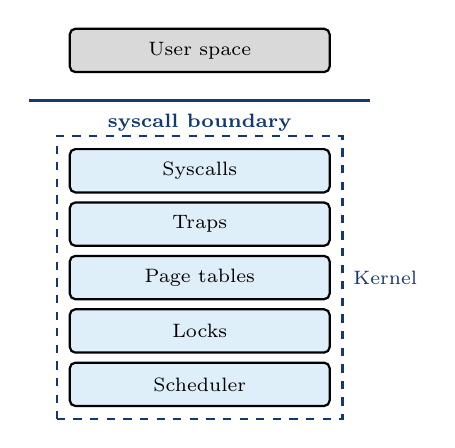
\begin{tikzpicture}[
          romanfont,
          box/.style={draw=utecblack,thick,rounded corners=2pt,fill=uteclight!25,
                      minimum width=3.3cm,minimum height=0.55cm,font=\scriptsize,align=center}]
        \node[box,fill=utecbggray] (us) {User space};
        \draw[utecnavy,very thick] ([yshift=-0.35cm, xshift=-0.5cm]us.south west) -- ([yshift=-0.35cm, xshift=0.5cm]us.south east)
              node[midway,below,font=\scriptsize\bfseries\color{utecnavy},yshift=-1pt] {syscall boundary};
        \node[box,below=0.95cm of us] (sc) {Syscalls};
        \node[box,below=0.1cm of sc] (tr) {Traps};
        \node[box,below=0.1cm of tr] (pt) {Page tables};
        \node[box,below=0.1cm of pt] (lk) {Locks};
        \node[box,below=0.1cm of lk] (sch) {Scheduler};
        \begin{pgfonlayer}{background}
          \node[draw=utecnavy,thick,dashed,inner sep=0.15cm,
                fit=(sc)(sch),label={[font=\scriptsize\color{utecnavy}]right:Kernel}] {};
        \end{pgfonlayer}
      \end{tikzpicture}
      \end{center}
  \end{columns}
\end{frame}

\begin{frame}{Background -- Extended Berkeley Packet Filters}
  \begin{itemize}
    \item User-provided programs loaded into the kernel, run at predefined hook points.
    \item Kernel verifies, optionally JIT-compiles, and runs them without touching the kernel binary.
  \end{itemize}
  \vspace{0.45cm}
  \resizebox{\textwidth}{!}{%
  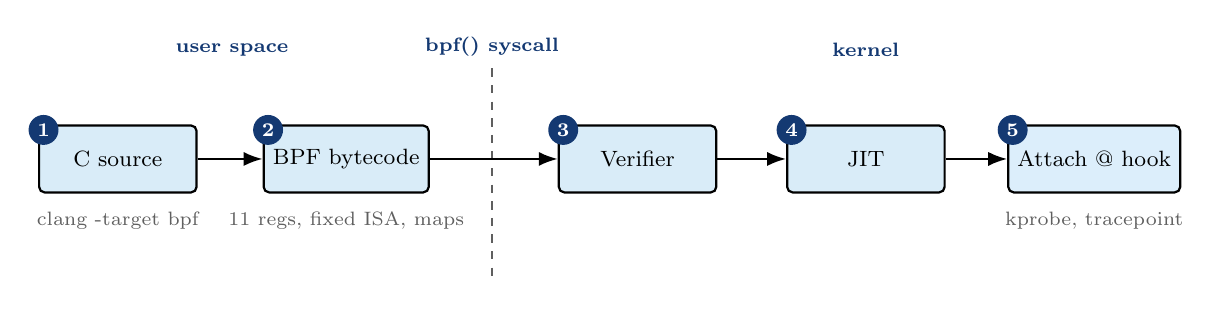
\begin{tikzpicture}[
      romanfont, font=\footnotesize,
      stage/.style={draw=utecblack,thick,rounded corners=2pt,fill=uteclight!30,
                    minimum width=2.0cm,minimum height=0.85cm,align=center},
      khook/.style={draw=utecblack,thick,rounded corners=2pt,fill=knTint,
                    minimum width=2.0cm,minimum height=0.85cm,align=center},
      note/.style={font=\scriptsize\color{utecgray},align=center},
      band/.style={font=\scriptsize\bfseries\color{utecnavy}},
      num/.style={circle,fill=utecnavy,text=white,inner sep=0pt,
                  minimum size=3.8mm,font=\scriptsize\bfseries},
      arr/.style={-{Latex[length=2.4mm]},thick,utecblack}]
    \node[stage] (src) at (0,0)    {C source};
    \node[stage] (bc)  at (2.9,0)  {BPF bytecode};
    \node[stage] (ver) at (6.6,0)  {Verifier};
    \node[stage] (jit) at (9.5,0)  {JIT};
    \node[khook] (hk)  at (12.4,0) {Attach @ hook};
    \node[num] at ([xshift=2pt,yshift=-2pt]src.north west) {1};
    \node[num] at ([xshift=2pt,yshift=-2pt]bc.north west)  {2};
    \node[num] at ([xshift=2pt,yshift=-2pt]ver.north west) {3};
    \node[num] at ([xshift=2pt,yshift=-2pt]jit.north west) {4};
    \node[num] at ([xshift=2pt,yshift=-2pt]hk.north west)  {5};
    \draw[utecgray,thick,dashed] (4.75,1.15) -- (4.75,-1.55);
    \node[band,anchor=south] at (4.75,1.18) {bpf() syscall};
    \node[band,anchor=south] at (1.45,1.18) {user space};
    \node[band,anchor=south] at (9.5,1.18) {kernel};
    \node[note,below=3pt of src] {clang -target bpf};
    \node[note,below=3pt of bc]  {11 regs, fixed ISA, maps};
    % \node[note,below=3pt of ver,text width=2.7cm] {bounded loops, memory safety, no leaks};
    % \node[note,below=3pt of jit] {to native code};
    \node[note,below=3pt of hk,text width=2.5cm]  {kprobe, tracepoint};
    \draw[arr] (src) -- (bc);
    \draw[arr] (bc)  -- (ver);
    \draw[arr] (ver) -- (jit);
    \draw[arr] (jit) -- (hk);
  \end{tikzpicture}}
\end{frame}

\begin{frame}[fragile]{Background -- A minimal eBPF program}

    \begin{figure}
        \centering
        \includegraphics[height=0.625\textheight]{ebpf.pdf}
    \end{figure}
\end{frame}

\begin{frame}{Background -- Static tracepoints and JIT}
  \textbf{\color{utecnavy}Static tracepoint}
  \begin{itemize}
    \item A named instrumentation point compiled into the kernel ahead of time.
    \item Idle until a program attaches, then it runs that program at exactly that point.
    \item Cheap to implement, unlike dynamic kprobes that rewrite running code.
  \end{itemize}
  \vspace{0.5cm}
  \textbf{\color{utecnavy}Just-in-time compilation}
  \begin{itemize}
    \item Translates a program's bytecode to native instructions at load time.
    \item Drops the per-instruction dispatch cost the interpreter pays on every run.
  \end{itemize}
\end{frame}

% =====================================================================
%  3.  RELATED WORK
% =====================================================================
\outlineslide{3}

\begin{frame}{Related Work}
  \scriptsize
  \renewcommand{\arraystretch}{1.75}
  \begin{tabular}{@{}>{\leavevmode\color{utecnavy}\bfseries}m{3.0cm} m{3.0cm} m{6.5cm}@{}}
    \toprule
    \leavevmode\color{utecnavy}\textbf{Work} & \color{utecnavy}\textbf{Focus} & \color{utecnavy}\textbf{Key finding} \\
    \midrule
    Ebling+ 2024 & OS teaching survey & Linux used by 62\% of OS instructors, xv6 by 17\%. \\
    Kuiter+ 2025 & Linux complexity & Feature count grew from 2,916 (2002) to 20,024 (2024), up to $10^{3600}$ valid configurations. \\
    \rowcolor{uteclight!25}
    Wen+ 2025 & KernelVM, browser VM & Snapshot recovery in $\sim$100 ms across 159 students, at a 10$\times$ compile slowdown. \\
    \rowcolor{uteclight!25}
    Zheng+ 2024 & KGENT, LLM eBPF synthesis & 80\% accuracy on 40 prompts, 2.67$\times$ over a GPT-4 baseline. \\
    Nelson+ 2020 & Jitterbug, JIT verification & Verified BPF JITs on 6 architectures, finding 16 previously unknown bugs. \\
    Gbadamosi+ 2024 & eBPF runtime survey & First end-to-end description of the eBPF runtime up to Linux v6.7. \\
    \bottomrule
  \end{tabular}
  \vskip2em
  \footnotesize
  \textcolor{utecnavy}{\textbf{Gap:}} no prior work brings eBPF-style runtime kernel extension into an educational kernel.
\end{frame}




% =====================================================================
%  4.  LUCUMAOS  -- overview, design space, then UI -> Toolchain -> Kernel
% =====================================================================
\outlineslide{4}

% --- System overview: the hero (navy) ---
\begin{frame}{LucumaOS -- System overview}
\vspace{-0.45cm}
\begin{figure}
    \centering
    \includegraphics[width=0.76\linewidth]{pfc-general-presentacion.pdf}
\end{figure}
\vspace{-0.25cm}
\takeaway{Three zones, one bridge: \hl{knZone}{guest kernel}, \hl{tcZone}{host toolchain}, \hl{uiZone}{user interface}, joined by an MMIO hypercall.}
\end{frame}


% =====================  KERNEL ZONE  (sky) -- guest / inside  =====================
\setbeamercolor{frametitle}{fg=white,bg=knDeep}

% \begin{frame}[fragile]{Kernel -- Static tracepoints in LucumaOS}
%   \minimap{minimap-kernel}
%   \begin{columns}[T]
%     \column{0.44\textwidth}
%       \footnotesize
%       \begin{itemize}\setlength{\itemsep}{7pt}
%         \item One macro plants a \textbf{\color{knDeep}named hook} in kernel source.
%         \item No runtime patching, no single-stepping.
%       \end{itemize}
%     \column{0.56\textwidth}
%       at the call site, in \texttt{kernel/proc.c}:
%       \begin{lstlisting}[style=cstyle]
% BPF_TRACE("sched_select", &ctx);
%       \end{lstlisting}
%       \vspace{0.25cm}
%       expands at compile time to:
%       \begin{lstlisting}[style=cstyle]
% if (bpf_active("sched_select"))
%     bpf_dispatch("sched_select", &ctx);
%       \end{lstlisting}
%   \end{columns}
% \end{frame}


\begin{frame}{Kernel -- Hook coverage}
  \takeaway{\hl{knDeep}{Static Hooks} sit in each of the five subsystems. One dispatcher serves them all.}
  \minimap{minimap-kernel}

  \vspace{-0.75cm}
  \begin{center}
  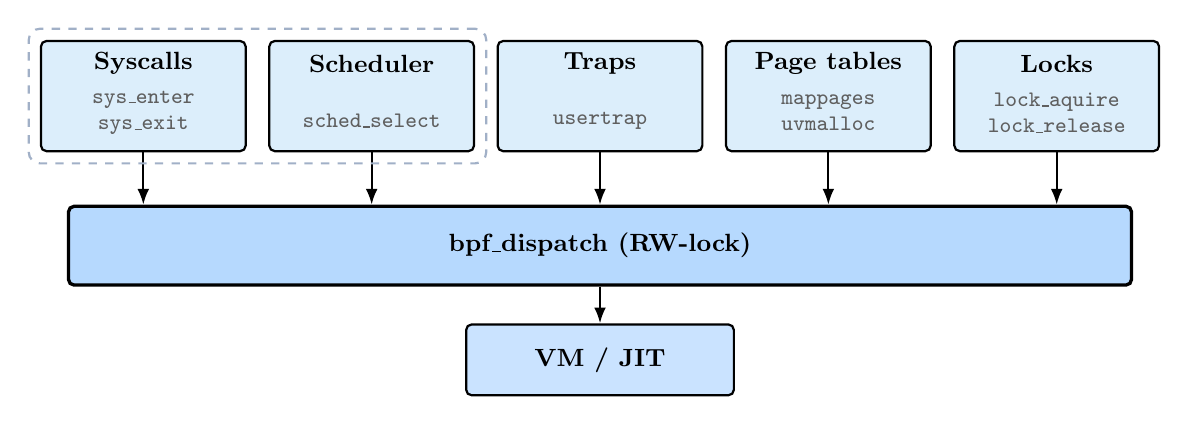
\begin{tikzpicture}[
      romanfont,
      region/.style={draw=utecblack,thick,rounded corners=2pt,fill=knTint,
                  minimum width=2.6cm,minimum height=1.4cm,align=center,inner sep=4pt},
      title/.style={font=\small\bfseries\color{utecblack}},
      hook/.style={font=\footnotesize\ttfamily\color{utecgray}},
      disp/.style={draw=utecblack,very thick,rounded corners=2pt,fill=knZone!55,
                  minimum width=13.5cm,minimum height=1.0cm,
                  font=\small\bfseries\color{utecblack},align=center},
      vmbox/.style={draw=black,thick,rounded corners=2pt,fill=knZone!40,
                  minimum width=3.4cm,minimum height=0.9cm,
                  font=\small\bfseries\color{utecblack},align=center},
      impl/.style={draw=utecnavy!40,thick,dashed,rounded corners,inner sep=4pt},
      arr/.style={-{Latex[length=2.0mm]},thick,utecblack}]
    \node[region] (sys) at (0,0)    {};
    \node[region] (sch) at (2.9,0)  {};
    \node[region] (tr)  at (5.8,0)  {};
    \node[region] (pt)  at (8.7,0)  {};
    \node[region] (lk)  at (11.6,0) {};
    \node[title] at ([yshift=-0.30cm]sys.north) {Syscalls};
    \node[title] at ([yshift=-0.30cm]sch.north) {Scheduler};
    \node[title] at ([yshift=-0.30cm]tr.north)  {Traps};
    \node[title] at ([yshift=-0.30cm]pt.north)  {Page tables};
    \node[title] at ([yshift=-0.30cm]lk.north)  {Locks};
    \node[hook,align=center] at ([yshift=0.50cm]sys.south) {sys\_enter\\sys\_exit};
    \node[hook,align=center] at ([yshift=0.40cm]sch.south) {sched\_select};
    \node[hook,align=center] at ([yshift=0.40cm]tr.south)  {usertrap};
    \node[hook,align=center] at ([yshift=0.50cm]pt.south)  {mappages\\uvmalloc};
    \node[hook,align=center] at ([yshift=0.50cm]lk.south)  {lock\_aquire\\lock\_release};
    \node[disp] (d) at (5.8,-1.9) {bpf\_dispatch (RW-lock)};
    \node[vmbox] (vm) at (5.8,-3.35) {VM / JIT};
    \draw[arr] (sys.south) -- (sys.south |- d.north);
    \draw[arr] (sch.south) -- (sch.south |- d.north);
    \draw[arr] (tr.south)  -- (tr.south  |- d.north);
    \draw[arr] (pt.south)  -- (pt.south  |- d.north);
    \draw[arr] (lk.south)  -- (lk.south  |- d.north);
    \draw[arr] (d) -- (vm);

    \node[impl,fit=(sys)(sch)] (implbox) {};
  \end{tikzpicture}
  \end{center}
\end{frame}


\begin{frame}{Kernel -- Execution and safety}
  \minimap{minimap-kernel}
  \begin{columns}[T]
    \column{0.46\textwidth}
      \footnotesize
      \begin{itemize}\setlength{\itemsep}{5pt}
        \item One syscall, \texttt{sys\_bpf}, with \texttt{LOAD} / \texttt{UNLOAD}; returns a program id to detach later.
        \item Dispatcher reads the registry under a \textbf{\color{knDeep}read-write lock}, so hooks in locked regions cannot deadlock.
        \item Programs run with \textbf{\color{knDeep}bounds-checked memory}, a \textbf{\color{knDeep}restricted call interface}, and a \textbf{\color{knDeep}hard iteration cap}.
        \item A faulting program is \textbf{\color{knDeep}auto-detached}.
      \end{itemize}
    \column{0.54\textwidth}
      \begin{center}
      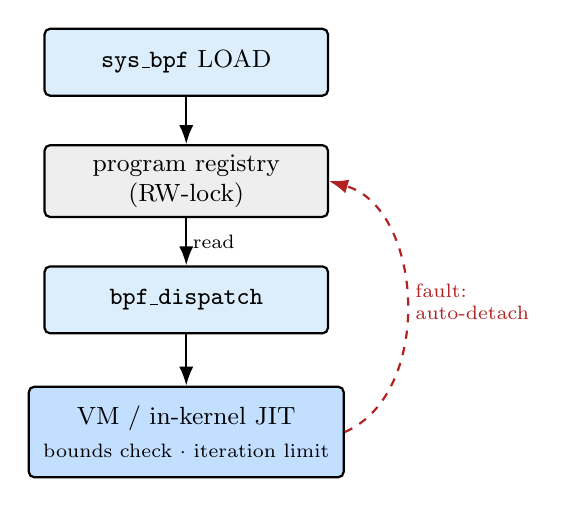
\begin{tikzpicture}[
          romanfont, font=\small,
          box/.style={draw=utecblack,thick,rounded corners=2pt,fill=knTint,
                      minimum width=3.6cm,minimum height=0.85cm,align=center},
          reg/.style={draw=utecblack,thick,rounded corners=2pt,fill=utecbggray!45,
                      minimum width=3.6cm,minimum height=0.9cm,align=center},
          exec/.style={draw=utecblack,thick,rounded corners=2pt,fill=knZone!45,
                      minimum width=4.0cm,minimum height=1.15cm,align=center},
          arr/.style={-{Latex[length=2.4mm]},thick,utecblack},
          darr/.style={-{Latex[length=2.4mm]},thick,probLabel,dashed}]
        \node[box] (load) {\texttt{sys\_bpf} LOAD};
        \node[reg,below=0.6cm of load] (reg) {program registry\\(RW-lock)};
        \node[box,below=0.6cm of reg] (disp) {\texttt{bpf\_dispatch}};
        \node[exec,below=0.65cm of disp] (vm) {VM / in-kernel JIT\\[1pt]\scriptsize bounds check $\cdot$ iteration limit};
        \draw[arr] (load) -- (reg);
        \draw[arr] (reg) -- node[right,font=\scriptsize\color{utecgray},inner sep=2pt]{read} (disp);
        \draw[arr] (disp) -- (vm);
        \draw[darr] (vm.east) to[bend right=70]
              node[right,font=\scriptsize\color{probLabel},align=left,inner sep=3pt]{fault:\\auto-detach} (reg.east);
      \end{tikzpicture}
      \end{center}
  \end{columns}
\end{frame}


\begin{frame}[fragile]{Kernel -- The luC dialect}
  \minimap{minimap-kernel}
  \begin{itemize}
    \item \textbf{\color{knDeep}luC} compiles to eBPF bytecode from \textbf{\color{knDeep}inside} the guest.
    \vskip0.9em
    \item Restrictions keep the compiler small and the bytecode verifiable:
      \begin{itemize}
        \item One function per file.
        \item All values 64-bit unsigned.
        \item Variables declared at the top.
      \end{itemize}
    \vskip0.9em
    \item Helpers exposed as built-in calls.
  \end{itemize}
\end{frame}

% luC lives here: the compiler ships INSIDE xv6-riscv.
\begin{frame}[fragile]{Kernel -- The luC dialect}
    \minimap{minimap-kernel}
    \begin{figure}
        \centering
        \includegraphics[height=0.55\textheight]{luc.pdf}
    \end{figure}
    \vskip1em
  \texttt{\$ luc heart.luc auto}\\
  \;\;\;\;\texttt{luc: 16 instructions -> hook 'sched\_select'}
\end{frame}


\begin{frame}{Kernel -- Running the bytecode}
  \minimap{minimap-kernel}
  Once luC emits bytecode, it runs in one of two ways:
  \vspace{0.4cm}
  \begin{columns}[T]
    \column{0.5\textwidth}
      \textbf{\color{knDeep}VM (interpreter)}
      \begin{itemize}
        \item Reads and executes one bytecode op at a time.
        \item Provides baseline safety.
      \end{itemize}
    \column{0.5\textwidth}
      \textbf{\color{knDeep}In-kernel JIT}
      \begin{itemize}
        \item Translates the bytecode to native RISC-V.
        \item Drops per-op dispatch.
      \end{itemize}
  \end{columns}
  \vspace{0.5cm}
  \takeaway{Same bytecode, two engines inside the guest. The \hl{tcDeep}{host LLVM JIT} adds a third, outside.}
\end{frame}


\begin{frame}{Kernel -- eBPF runtime}
\minimap{minimap-kernel}
\vspace{-0.77cm}
\begin{figure}
    \centering
    \includegraphics[width=0.69\linewidth]{pfc-kernel.pdf}
\end{figure}
\end{frame}


% =====================  TOOLCHAIN ZONE  (sage) -- host / outside  =====================
\setbeamercolor{frametitle}{fg=white,bg=tcDeep}

\begin{frame}{Toolchain -- Host LLVM JIT}
  \minimap{minimap-tools}
  \vspace{-0.1cm}
  \begin{center}
  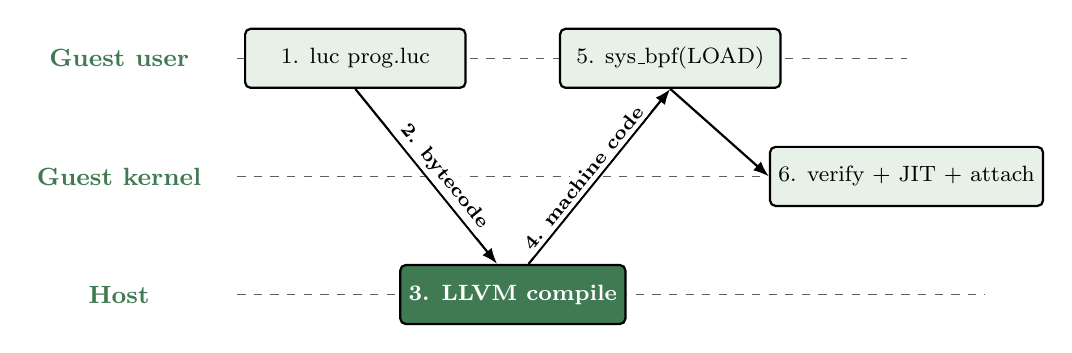
\begin{tikzpicture}[
      romanfont,
      lanew/.style={font=\small\bfseries\color{tcDeep}},
      stepbox/.style={draw=utecblack,thick,rounded corners=2pt,fill=tcTint,
                  minimum width=2.8cm,minimum height=0.75cm,
                  font=\footnotesize,align=center,inner sep=3pt},
      stepbox2/.style={draw=utecblack,thick,rounded corners=2pt,fill=tcDeep,
                  minimum width=2.8cm,minimum height=0.75cm,
                  font=\footnotesize\color{white},align=center,inner sep=3pt},
      arr/.style={-{Latex[length=2.0mm]},thick,utecblack},
      arrlbl/.style={font=\scriptsize\color{utecgray},inner sep=1.5pt, fill=white}]
    \node[lanew] (l1) at (0,0) {Guest user};
    \node[lanew] (l2) at (0,-1.5) {Guest kernel};
    \node[lanew] (l3) at (0,-3.0) {Host};
    \draw[utecgray,dashed] (1.5,0)    -- (10,0);
    \draw[utecgray,dashed] (1.5,-1.5) -- (11,-1.5);
    \draw[utecgray,dashed] (1.5,-3.0) -- (11,-3.0);
    \node[stepbox] (s1) at (3.0,0)    {1. luc prog.luc};
    \node[stepbox2] (s2) at (5.0,-3.0) {\textbf{3. LLVM compile}};
    \node[stepbox] (s3) at (7.0,0)    {5. sys\_bpf(LOAD)};
    \node[stepbox] (s4) at (10.0,-1.5) {6. verify + JIT + attach};
    \draw[arr] (s1.south) -- node[arrlbl,sloped,above,pos=0.55] {\textbf{2. bytecode}} ($(s2.north)+(-0.2,0)$);
    \draw[arr] ($(s2.north)+(0.2,0)$) -- node[arrlbl,sloped,above,pos=0.45] {\textbf{4. machine code}} (s3.south);
    \draw[arr] (s3.south) -- (s4.west);
  \end{tikzpicture}
  \end{center}
  \vskip0.6em
  \takeaway{Compilation is \hl{tcDeep}{offloaded to LLVM} over a hypercall, so xv6-riscv never carries a full toolchain.}
\end{frame}

\begin{frame}[fragile]{Toolchain -- Host C compiler}
  \minimap{minimap-tools}
  \begin{itemize}
    \item The host toolchain also compiles \textbf{\color{tcDeep}ordinary C}, beyond luC and bytecode.
    \item Clang targets RISC-V; the ELF returns through the inbox and runs.
  \end{itemize}
  \vskip5em
  \takeaway{The same outside boundary now serves \hl{tcDeep}{full C programs}, with no compiler inside xv6.}
\end{frame}



% =====================  UI ZONE  (rose) -- the GUI, two-column with callouts  =====================
\setbeamercolor{frametitle}{fg=white,bg=uiDeep}
% TODO: verify each numbered callout below matches the red circles in your figure.

\begin{frame}{Interface -- Console}
  \minimapbr{minimap-ui}
  \begin{columns}[T]
    \column{0.72\textwidth}
      \centering
      \includegraphics[width=\linewidth]{figs/console.pdf}
    \column{0.28\textwidth}
      \scriptsize
      \textbf{\color{uiZone}The operator's terminal into the running guest.}
      \vspace{0.3cm}

      \textbf{\color{uiZone}1.}~Shell input. Type commands straight into xv6.
      \vspace{0.4cm}

      Tabs switch Console / Inbox / Events / Memory.
      \vspace{0.4cm}
      
      Dots show socket status.
  \end{columns}
\end{frame}

\begin{frame}{Interface -- Inbox}
  \minimapbr{minimap-ui}
  \begin{columns}[T]
    \column{0.72\textwidth}
      \centering
      \includegraphics[width=\linewidth]{figs/inbox.pdf}
    \column{0.28\textwidth}
      \scriptsize
      \textbf{\color{uiZone}Send a luC program into the guest.}
      \vspace{0.3cm}

      \textbf{\color{uiZone}1.}~Destination path inside the guest.
      \vspace{0.18cm}

      \textbf{\color{uiZone}2.}~Payload type: luC source or raw file.
      \vspace{0.18cm}

      \textbf{\color{uiZone}3.}~Send (Ctrl+Enter).
  \end{columns}
\end{frame}

\begin{frame}{Interface -- Events}
  \minimapbr{minimap-ui}
  \begin{columns}[T]
    \column{0.72\textwidth}
      \centering
      \includegraphics[width=\linewidth]{figs/event.pdf}
    \column{0.28\textwidth}
      \scriptsize
      \textbf{\color{uiZone}Trace output streamed back.}
      \vspace{0.3cm}

      Every \texttt{trace\_print} from an attached program arrives here, timestamped and live.
  \end{columns}
\end{frame}

\begin{frame}{Interface -- Memory}
  \minimapbr{minimap-ui}
  \begin{columns}[T]
    \column{0.72\textwidth}
      \centering
      \includegraphics[width=\linewidth]{figs/memory.pdf}
    \column{0.28\textwidth}
      \scriptsize
      \textbf{\color{uiZone}Read kernel memory on demand.}
      \vspace{0.3cm}

      \textbf{\color{uiZone}1.}~Kernel address, in hex.
      \vspace{0.18cm}

      \textbf{\color{uiZone}2.}~Dump that many bytes of direct-mapped RAM.
  \end{columns}
\end{frame}


% =====================================================================
%  5.  EVALUATION AND RESULTS
% =====================================================================
\setbeamercolor{frametitle}{fg=white,bg=utecnavy}

\outlineslide{5}

\begin{frame}[fragile]{Evaluation -- End-to-end demos}
  \begin{columns}[T]
    \column{0.5\textwidth}
      \textbf{\color{utecnavy}Demo 1: luC arithmetic}
      \begin{itemize}
        \item Six-line luC program compiles, loads on \texttt{sched\_select}, prints periodically.
        \item Exercises source $\rightarrow$ host compile $\rightarrow$ guest load $\rightarrow$ hook fire.
      \end{itemize}
      \vspace{0.2cm}
      \scriptsize
      \begin{lstlisting}[style=lucstyle]
$ luc arith.luc auto
luc: 42 instructions
   -> hook 'sched_select'
BPF Trace: 107   // 100 + 7
BPF Trace: 93    // 100 - 7
BPF Trace: 700   // 100 * 7
      \end{lstlisting}
    \column{0.5\textwidth}
      \textbf{\color{utecnavy}Demo 2: Scheduler replacement}
      \begin{itemize}
        \item Attached program returns the pid to run on each \texttt{sched\_select} fire.
        \item Swapping the program changes policy at runtime, no kernel rebuild.
      \end{itemize}
      \vspace{0.2cm}
      \scriptsize
      \centering
      \begin{tabular}{@{}l l@{}}
        \toprule
        \color{utecnavy}\textbf{Policy} & \color{utecnavy}\textbf{Execution trace} \\
        \midrule
        Round Robin & ABCDEFG\,ABCDEFG \\
        Random      & ABCDEFG\,AECEAGA \\
        Max PID     & ABCDEFG\,GGGGGGG \\
        \bottomrule
      \end{tabular}
  \end{columns}
\end{frame}

\begin{frame}{Evaluation -- JIT performance}
  \begin{table}[h]
    \centering
    \renewcommand{\arraystretch}{1.2}
    \begin{tabular}{l c c c}
      \toprule
      \rowcolor{utecnavy}
      \color{white}\textbf{Mode} & \color{white}\textbf{Ticks $\downarrow$} & \color{white}\textbf{Wall time $\downarrow$} & \color{white}\textbf{Throughput $\uparrow$} \\
      Interpreter & 6 & $\sim$60 ms & $\sim$250 M ins/s \\
      \rowcolor{knTint}
      \textbf{JIT} & \textbf{1} & $\sim$\textbf{10 ms} & $\sim$\textbf{1.5 G ins/s} \\
      \bottomrule
    \end{tabular}
    \caption{\footnotesize Performance: 15M-instruction ALU loop.}
  \end{table}
  \begin{table}[h]
    \centering
    \renewcommand{\arraystretch}{1.2}
    \small
    \begin{tabular}{l c c c c}
      \rowcolor{utecnavy}
      \color{white}\textbf{Test} & \color{white}\textbf{BPF insns} & \color{white}\textbf{In-kernel JIT $\downarrow$} & \color{white}\textbf{Host JIT $\downarrow$} & \color{white}\textbf{Ratio $\uparrow$} \\
      A: stack store/load & 8 & 364 B & \textbf{152 B} & 2.39$\times$ \\
      B: div-by-zero (fault) & 4 & 188 B & \textbf{32 B} & 5.88$\times$ \\
      C: loop sum 1..1000 & 6 & 216 B & \textbf{12 B} & 18.0$\times$\textsuperscript{*} \\
      \bottomrule
    \end{tabular}
    \caption{\footnotesize Code size: In-kernel JIT vs Host JIT (LLVM). \textsuperscript{*}LLVM folded it to a closed form.}
  \end{table}
  \vspace{0.1cm}
  \takeaway{Host JIT keeps the 6$\times$ speedup while cutting code size.}
\end{frame}

\begin{frame}{Evaluation -- Readability cost}

  How many \textbf{kernel} Lines of Code (LoC) are added to the kernel by each backend.

  \vskip1.5em
  \renewcommand{\arraystretch}{1.4}
  \begin{center}
  \begin{tabular}{@{}>{\leavevmode\color{utecnavy}\bfseries}m{3.2cm} c c@{}}
    \rowcolor{utecnavy}
     & \color{white}\textbf{In-kernel LoC $\downarrow$}
     & \color{white}\textbf{Off-kernel LoC} \\
    Interpreter   & 262 & - \\
    In-kernel JIT & 575 & - \\
    \rowcolor{knTint}
    Host LLVM JIT & \textbf{273} & 1032 \\
    \bottomrule
  \end{tabular}
  \end{center}
  \vskip1.5em
  \takeaway{Same 6$\times$ speedup, but Host JIT adds \hl{knDeep}{half the LoC.}}
\end{frame}

% =====================================================================
%  6.  CONCLUSIONS
% =====================================================================
\outlineslide{6}

\begin{frame}{Conclusions}
  \execblock{ideaLabel}{ideaBG}{%
    \textcolor{ideaLabel}{\textbf{\underline{Conclusion 1:}}}
    The core idea of eBPF, \textcolor{ideaLabel}{\textbf{runtime kernel extension under safety constraints}},
    fits an educational kernel at a tractable engineering cost.}
  \execblock{ideaLabel}{ideaBG}{%
    \textcolor{ideaLabel}{\textbf{\underline{Conclusion 2:}}}
    The mechanism on xv6-riscv
    \textcolor{ideaLabel}{\textbf{removes the edit-rebuild-reboot loop}}
    for kernel experiments.}
  \execblock{ideaLabel}{ideaBG}{%
    \textcolor{ideaLabel}{\textbf{\underline{Conclusion 3:}}}
    The system stays \textcolor{ideaLabel}{\textbf{small enough to read and modify}},
    while preserving conceptual fidelity to production eBPF.}
  \vspace{0.2cm}
  \takeaway{A student can change kernel behavior in \hl{knDeep}{runtime}, not a \hl{probLabel}{rebuild cycle}.}
\end{frame}

\begin{frame}{Future Work}
    \execblock{resLabel}{resBG}{%
      \textcolor{resLabel}{\textbf{\underline{Extend hook coverage:}}}
      Add tracepoints for Traps, Locks, and Page Tables.}
    \execblock{resLabel}{resBG}{%
      \textcolor{resLabel}{\textbf{\underline{LLM-assisted authoring:}}}
      Use a language model to help students write and debug luC programs.}
    \execblock{resLabel}{resBG}{%
      \textcolor{resLabel}{\textbf{\underline{Richer kernel features:}}}
      Implement non-trivial kernel subsystems entirely via eBPF programs.}
\end{frame}

% =====================================================================
%  APPENDIX
% =====================================================================
\begin{frame}{References}
  \scriptsize
  \begin{thebibliography}{99}
    \bibitem{ebling2024} Ebling, M. R. (2024). Resources for teaching operating systems: A survey of instructors and a literature review. \textit{ACM Transactions on Computing Education}, 24(4).
    \bibitem{kuiter2025} Kuiter, E., Sundermann, C., Th\"um, T., He{\ss}, T., Krieter, S., \& Saake, G. (2025). How configurable is the Linux kernel? \textit{ACM Computing Surveys}.
    \bibitem{nieh2025} Nieh, E., Zhang, Z., \& Nieh, J. (2025). ezFS: a pedagogical Linux file system. \textit{SIGCSE}.
    \bibitem{wen2025} Wen, E., Ma, S., Denny, P., Tempero, E., Weber, G., \& Yue, K. (2025). KernelVM: teaching Linux kernel programming through a browser-based virtual machine. \textit{SIGCSE}.
    \bibitem{zheng2024} Zheng, Y., Yang, Y., Chen, M., \& Quinn, A. (2024). KGent: Kernel extensions large language model agent. \textit{eBPF Workshop}.
    \bibitem{nelson2020} Nelson, L., Van Geffen, J., Torlak, E., \& Wang, X. (2020). Specification and verification in the field: applying formal methods to BPF just-in-time compilers in the Linux kernel. \textit{OSDI}.
    \bibitem{gbadamosi2024} Gbadamosi, et al. (2024). A comprehensive description of the eBPF runtime in the Linux kernel. arXiv:2410.00026.
    \bibitem{jia2023} Jia, J., et al. (2023). Programmable system call security with eBPF. arXiv:2302.10366.
  \end{thebibliography}
\end{frame}

\begin{frame}{Repository and Disclaimer}

\textbf{Github Repository:} \\
\url{https://github.com/slamgLuke/xv6-riscv-bpf}

\vskip3em

\textbf{Disclaimer:} Parts of LucumaOS where developed using Generative AI:
\begin{itemize}
    \item QEMU MMIO device, GUI, and JIT test suite were generated using AI.
    \item The in-kernel and host JIT backends, the verifier, and the dispatch path were developed with AI assistance.
\end{itemize}
\end{frame}

\end{document}